\documentclass{article}
\usepackage{graphicx} %package to manage images
\usepackage[utf8]{inputenc}
\usepackage[a4paper, total={6in, 8in}]{geometry}
\usepackage{xurl}
\usepackage{hyperref}
\usepackage{float}
\title{Relatório 16 \\ ROC curves}
\author{Pedro A. S. O. Neto}
\date{Dezembro, 2023}

\begin{document}

\maketitle

\section{Pré-pos ANOVAS}

Descriptive of the sample. 

\begin{table}[ht]
\centering
\begin{tabular}{rlllrrr}
  \hline
 & sexo & tea & prePos & sdAgeJA & meanAgeJA & N \\ 
  \hline
1 & F & TD & post & 0.59 & 2.21 &   7 \\ 
  2 & F & TD & pre & 1.02 & 2.79 & 260 \\ 
  3 & F & TEA & post &  & 2.00 &   1 \\ 
  4 & F & TEA & pre & 0.92 & 2.06 &   3 \\ 
  5 & F & nonTD & pre & 1.30 & 2.85 &  10 \\ 
  6 & F & other & pre & 1.59 & 2.54 &   2 \\ 
  7 & F &  & pre & 1.06 & 3.38 &   4 \\ 
  8 & M & TD & post & 0.55 & 2.51 &  17 \\ 
  9 & M & TD & pre & 1.09 & 2.66 & 274 \\ 
  10 & M & TEA & post & 1.00 & 2.99 &  25 \\ 
  11 & M & TEA & pre & 0.89 & 3.11 &  37 \\ 
  12 & M & nonTD & pre & 0.83 & 3.07 &  13 \\ 
  13 & M & other & post & 0.47 & 2.58 &   2 \\ 
  14 & M & other & pre & 0.54 & 3.04 &   7 \\ 
  15 & M &  & pre & 0.91 & 3.22 &   9 \\ 
  16 & nan &  & pre &  &  &   4 \\ 
   \hline
\end{tabular}
\end{table}

\section{Alternâncias}

\begin{figure}[H]
  \caption{ANOVA alternancias. Main effect of pre-pos}
  \noindent\makebox[\textwidth]{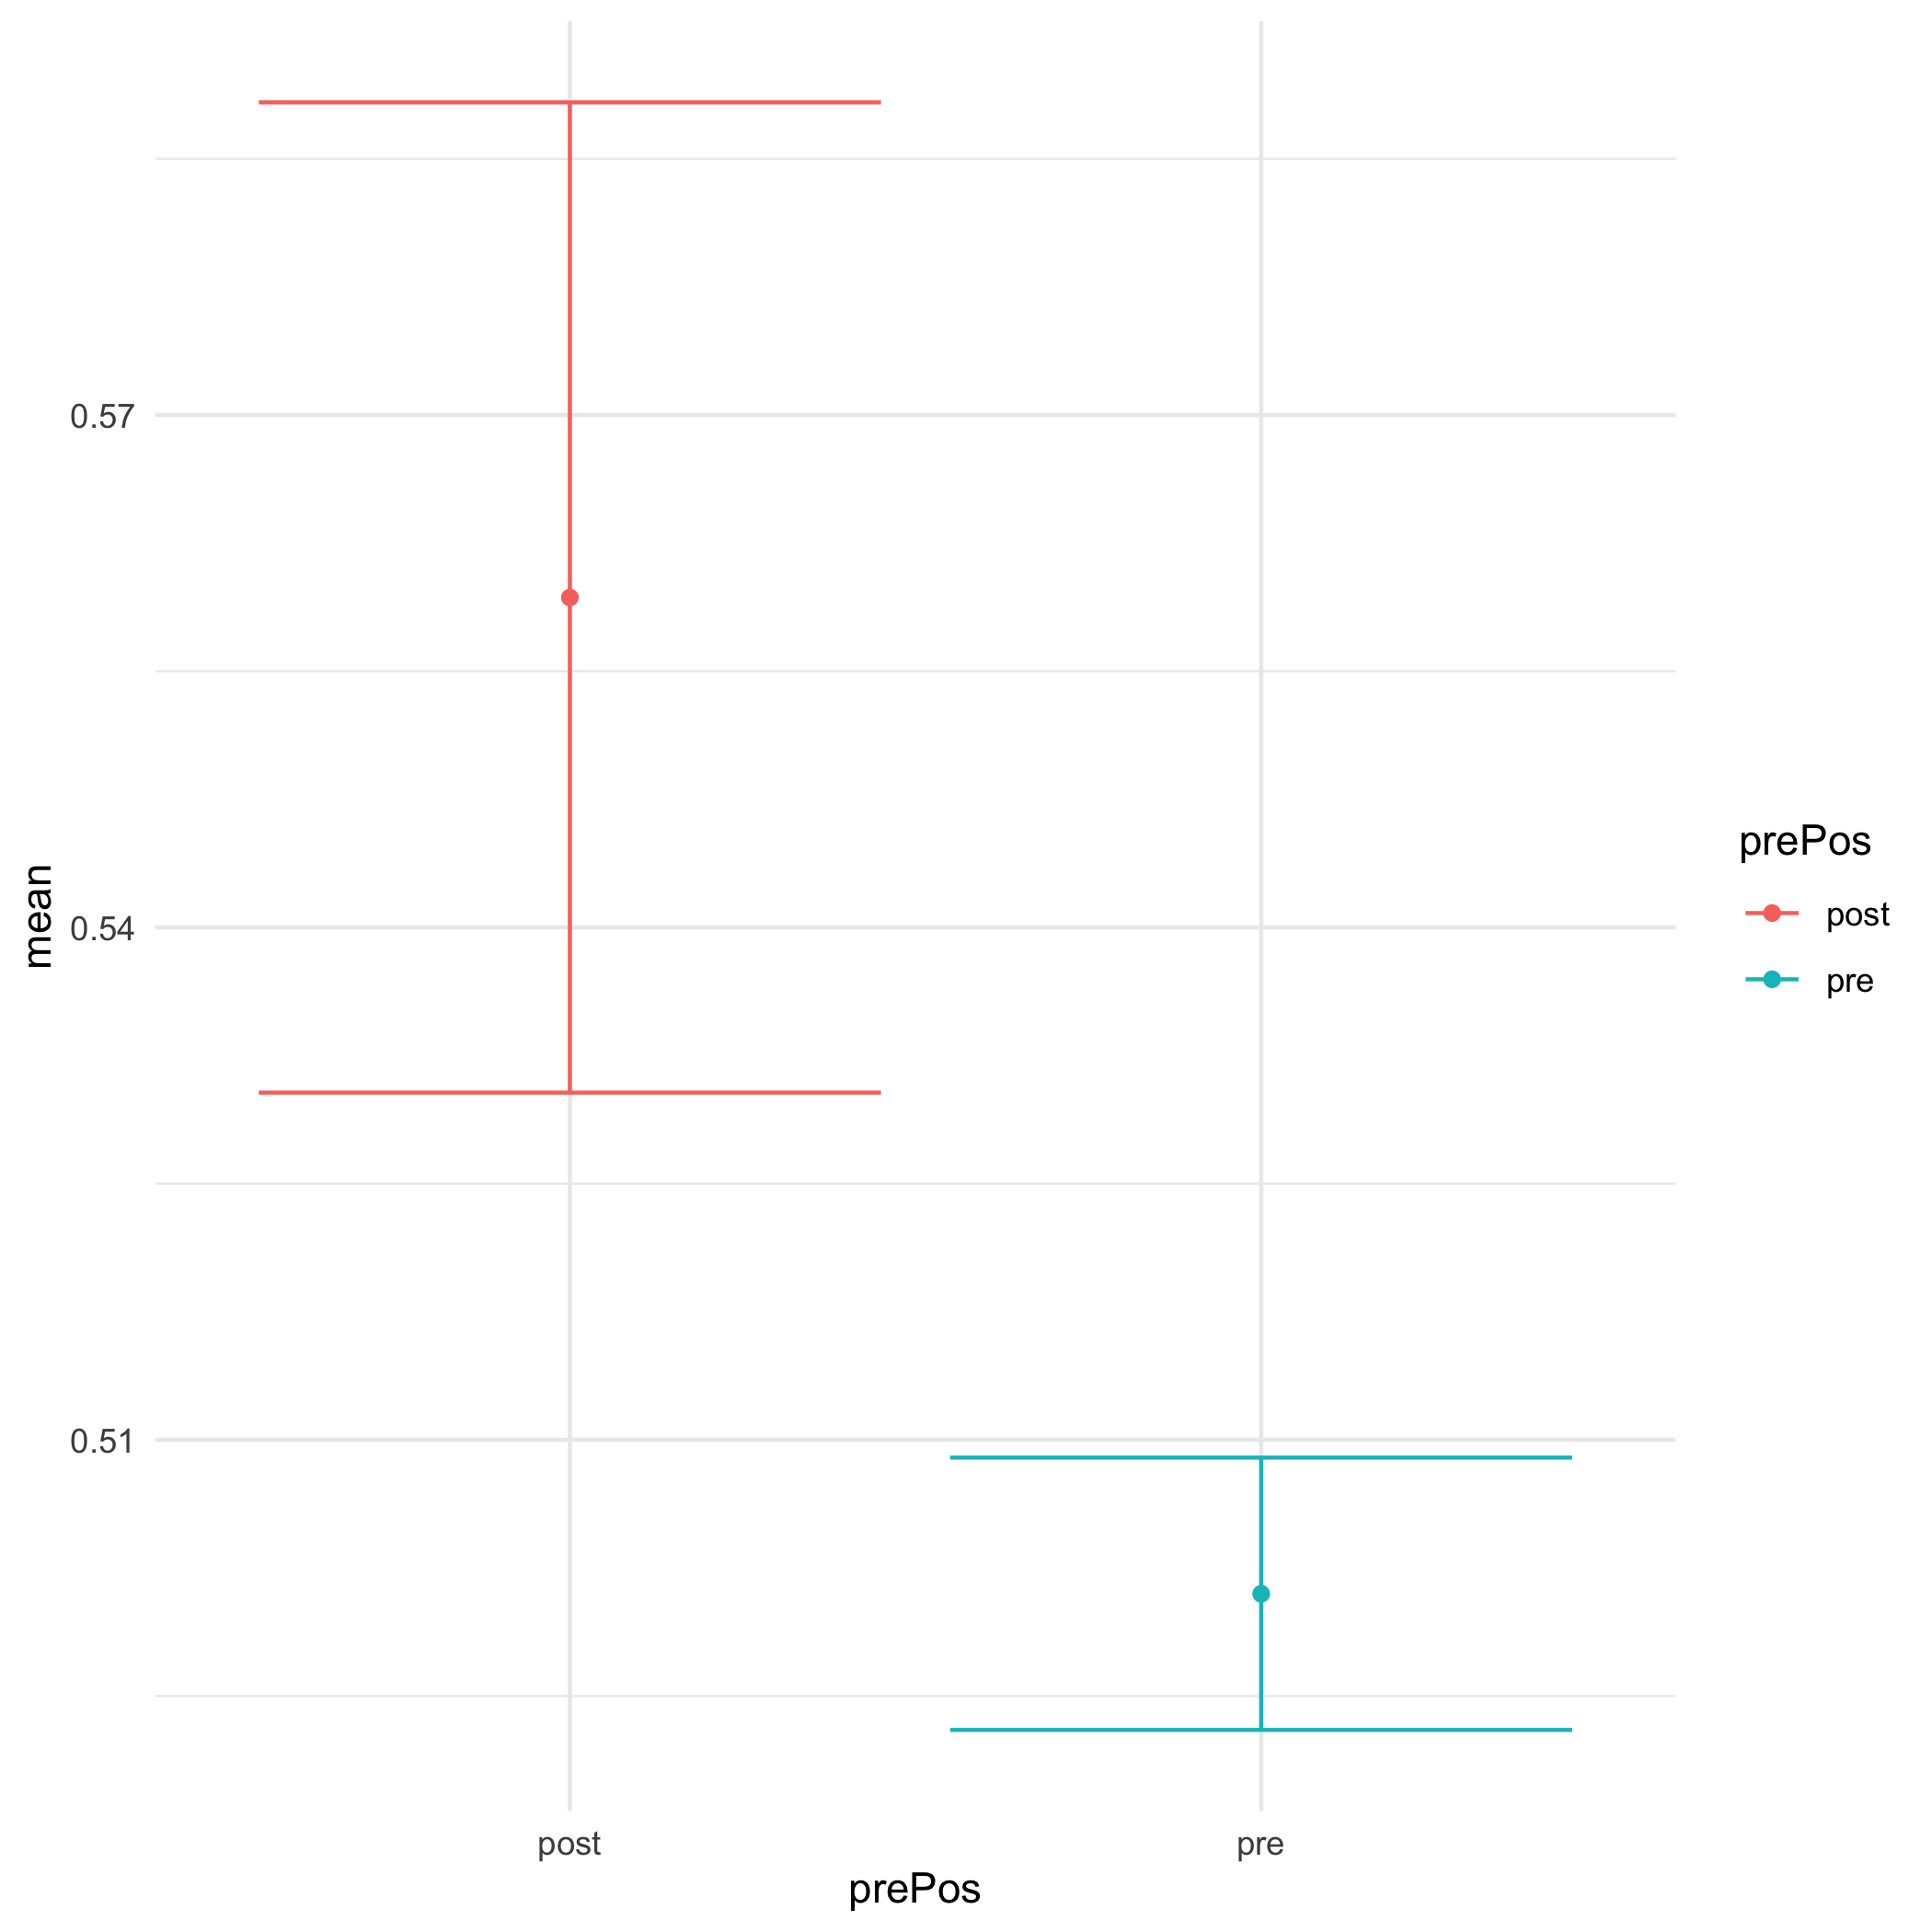
\includegraphics[scale=0.2]{./prePos.png}}
  \centering
\end{figure}

\begin{table}[ht]
\centering
\begin{tabular}{rlrr}
  \hline
 & prePos & mean & stder \\ 
  \hline
  1 & post & 0.56 & 0.03 \\ 
  2 & pre & 0.50 & 0.01 \\ 
   \hline
\end{tabular}
\end{table}

\begin{figure}[H]
  \caption{Interaction of PrePost and variable on alternancias}
  \noindent\makebox[\textwidth]{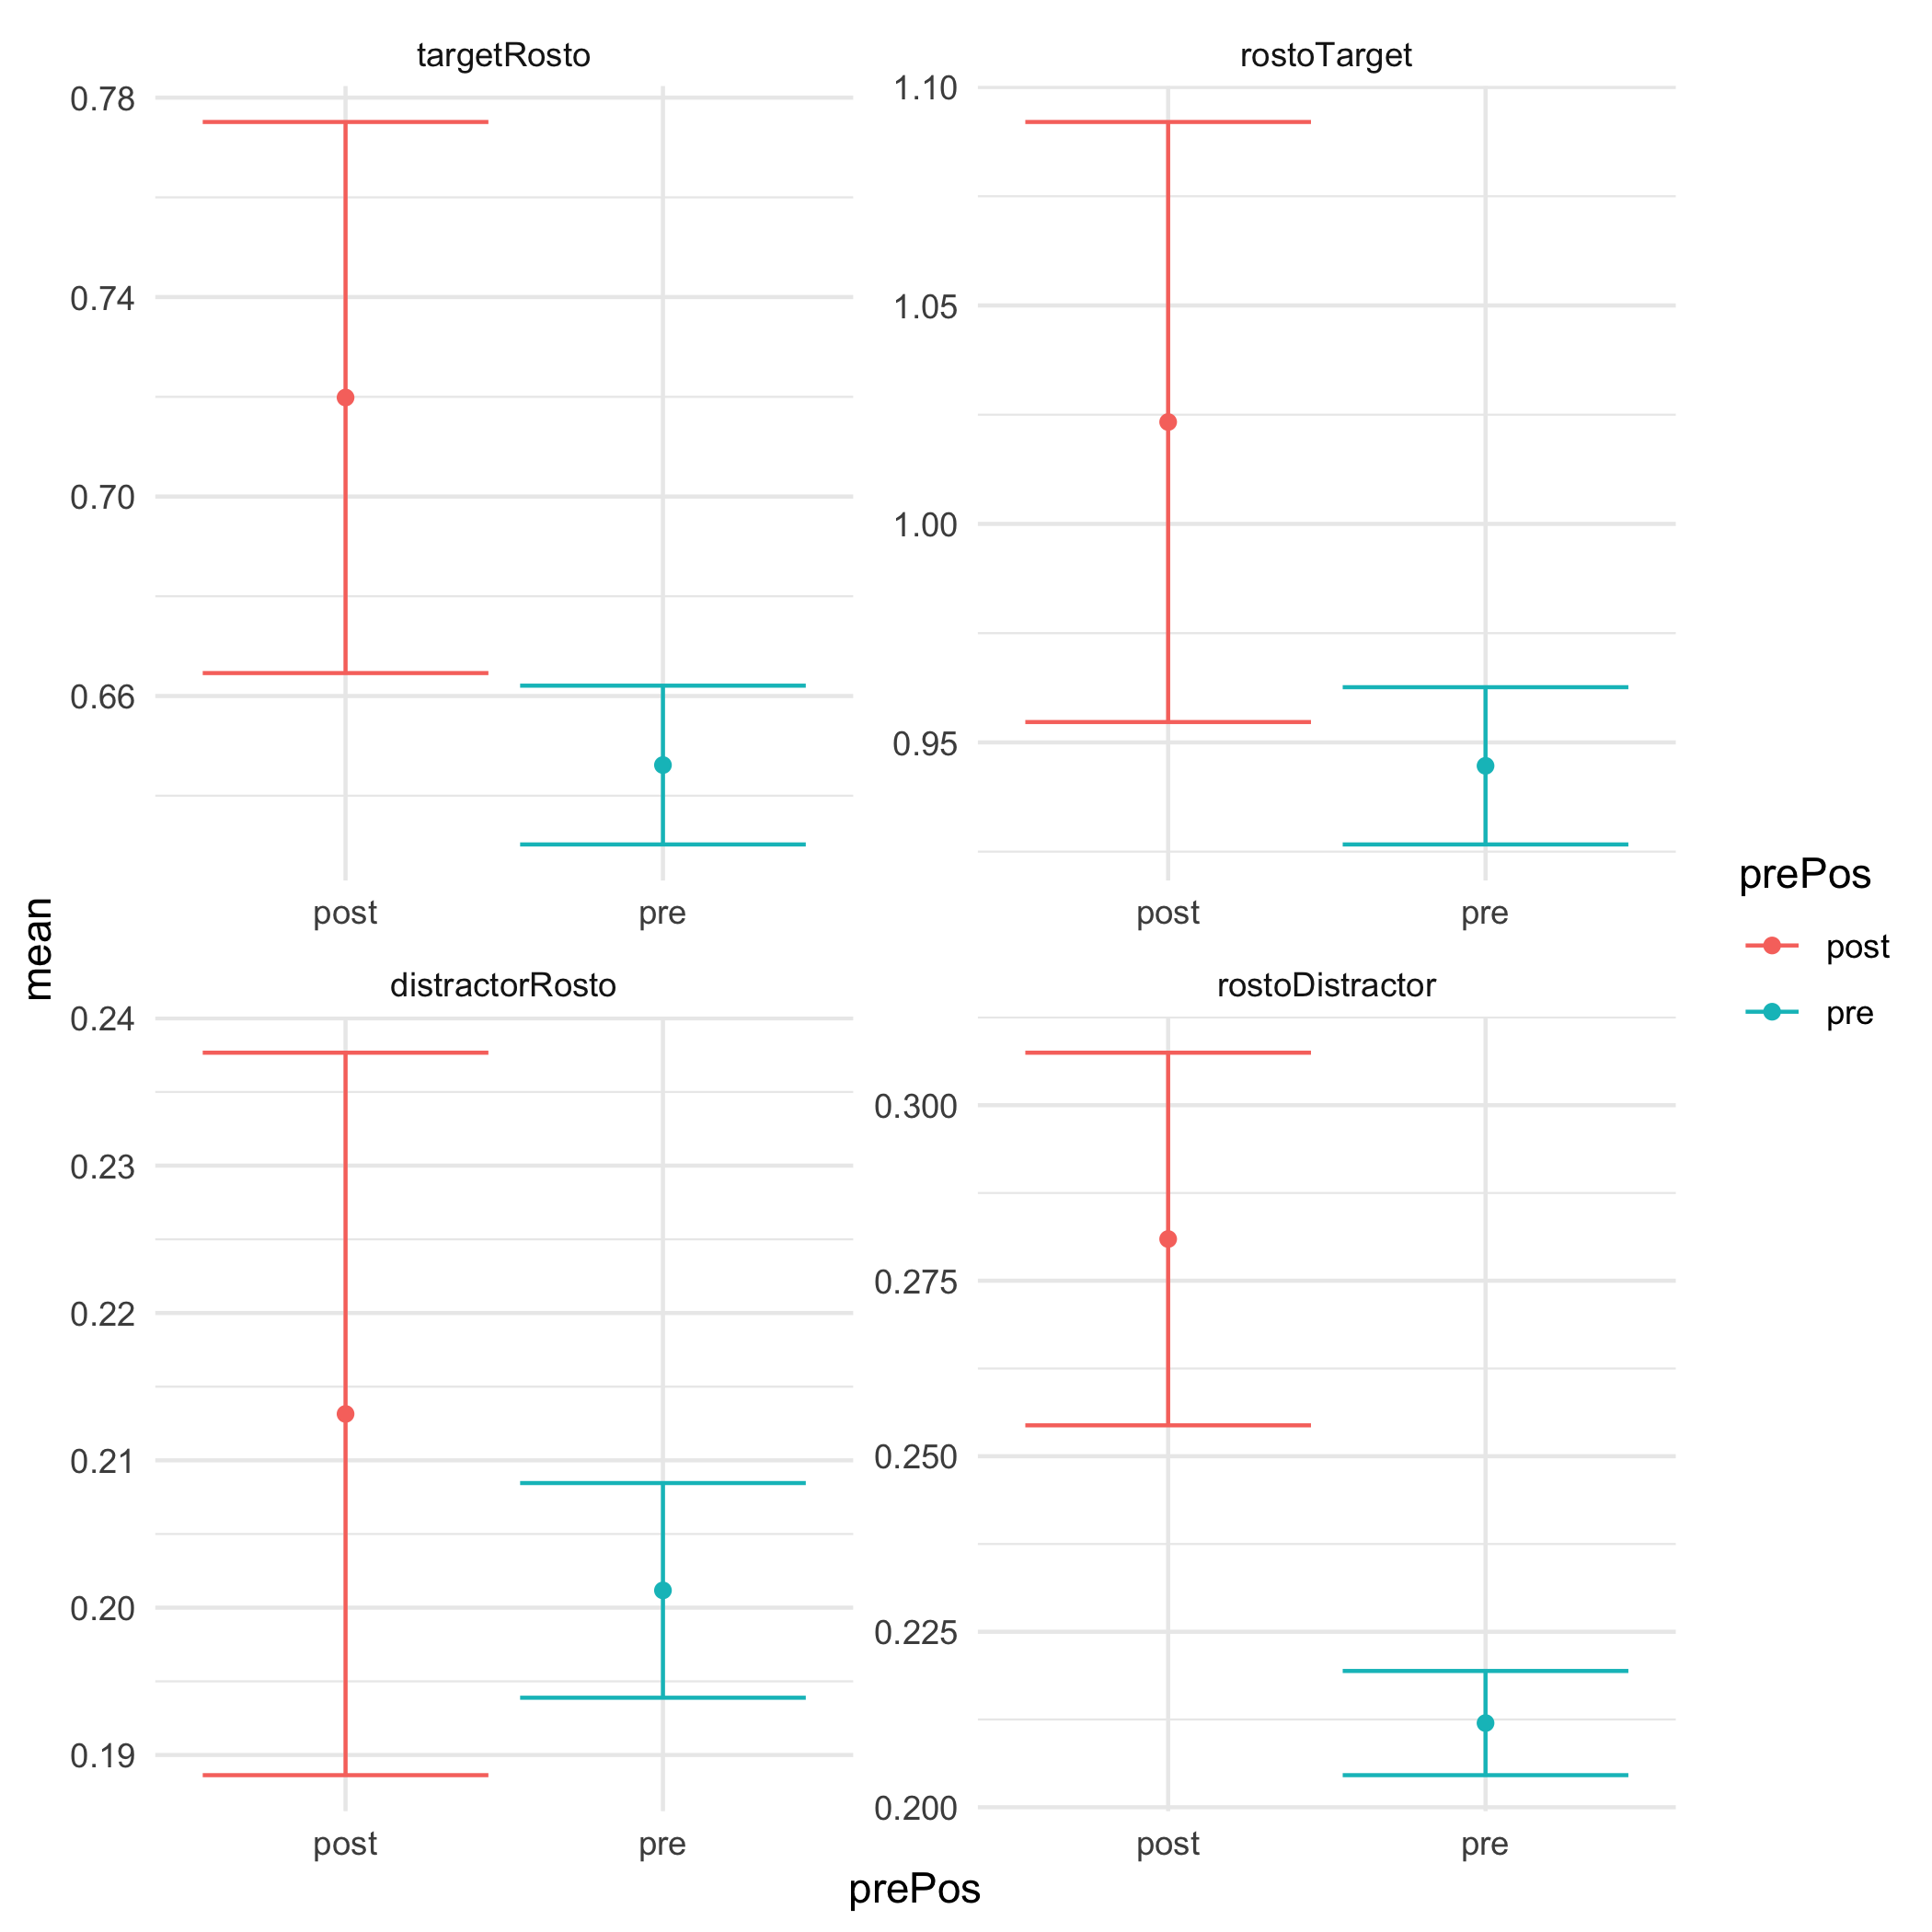
\includegraphics[scale=0.2]{./prePosVar.png}}
  \centering
\end{figure}

\begin{table}[ht]
\centering
\begin{tabular}{rllrr}
  \hline
 & prePos & variable & mean & stder \\ 
  \hline
1 & post & targetRosto & 0.72 & 0.06 \\ 
  2 & post & rostoTarget & 1.02 & 0.07 \\ 
  3 & post & distractorRosto & 0.21 & 0.02 \\ 
  4 & post & rostoDistractor & 0.28 & 0.03 \\ 
  5 & pre & targetRosto & 0.65 & 0.02 \\ 
  6 & pre & rostoTarget & 0.94 & 0.02 \\ 
  7 & pre & distractorRosto & 0.20 & 0.01 \\ 
  8 & pre & rostoDistractor & 0.21 & 0.01 \\ 
   \hline
\end{tabular}
\end{table}


\begin{figure}[H]
  \caption{Interaction between pre, post and condition on alternancias.}
  \noindent\makebox[\textwidth]{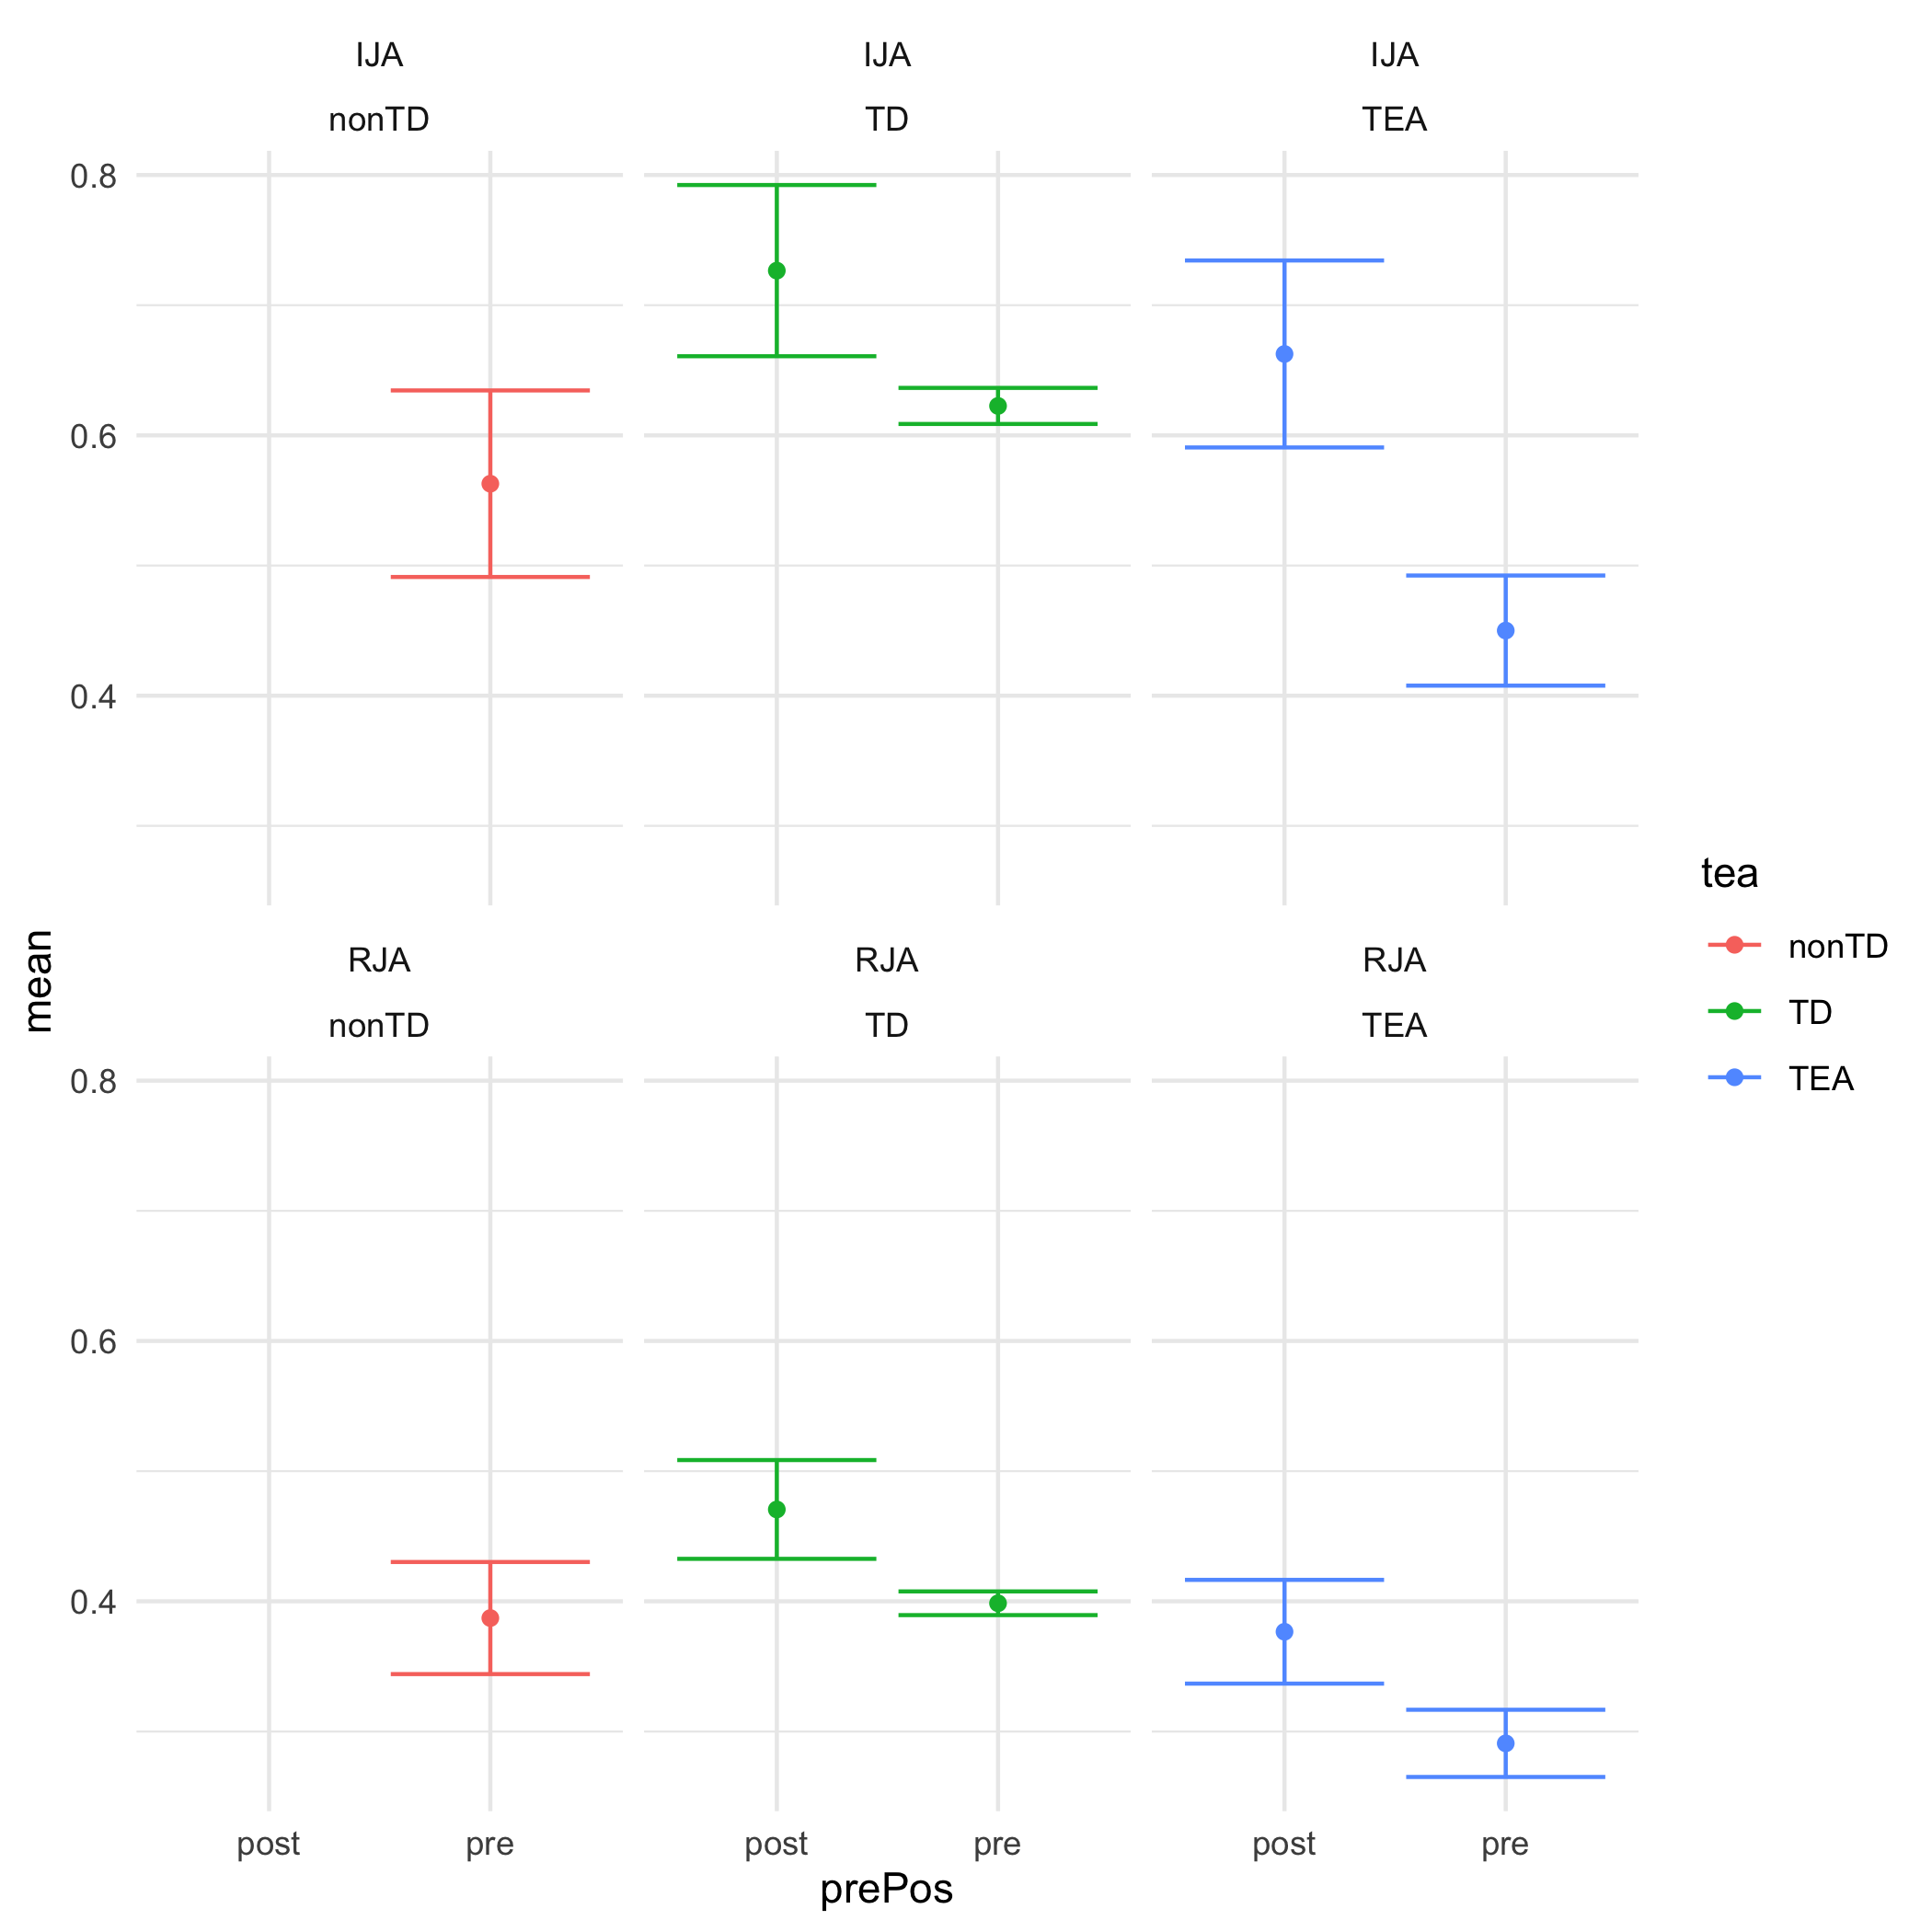
\includegraphics[scale=0.2]{./prePosCondition.png}}
  \centering
\end{figure}

\begin{table}[ht]
\centering
\begin{tabular}{rlllrr}
  \hline
 & tea & prePos & condition & mean & stder \\ 
  \hline
1 & nonTD & pre & IJA & 0.56 & 0.07 \\ 
  2 & nonTD & pre & RJA & 0.39 & 0.04 \\ 
  3 & TD & post & IJA & 0.73 & 0.07 \\ 
  4 & TD & post & RJA & 0.47 & 0.04 \\ 
  5 & TD & pre & IJA & 0.62 & 0.01 \\ 
  6 & TD & pre & RJA & 0.40 & 0.01 \\ 
  7 & TEA & post & IJA & 0.66 & 0.07 \\ 
  8 & TEA & post & RJA & 0.38 & 0.04 \\ 
  9 & TEA & pre & IJA & 0.45 & 0.04 \\ 
  10 & TEA & pre & RJA & 0.29 & 0.03 \\ 
   \hline
\end{tabular}
\end{table}

\section{Proportions}

\begin{figure}[H]
  \caption{PrePos variable effect on variable}
  \noindent\makebox[\textwidth]{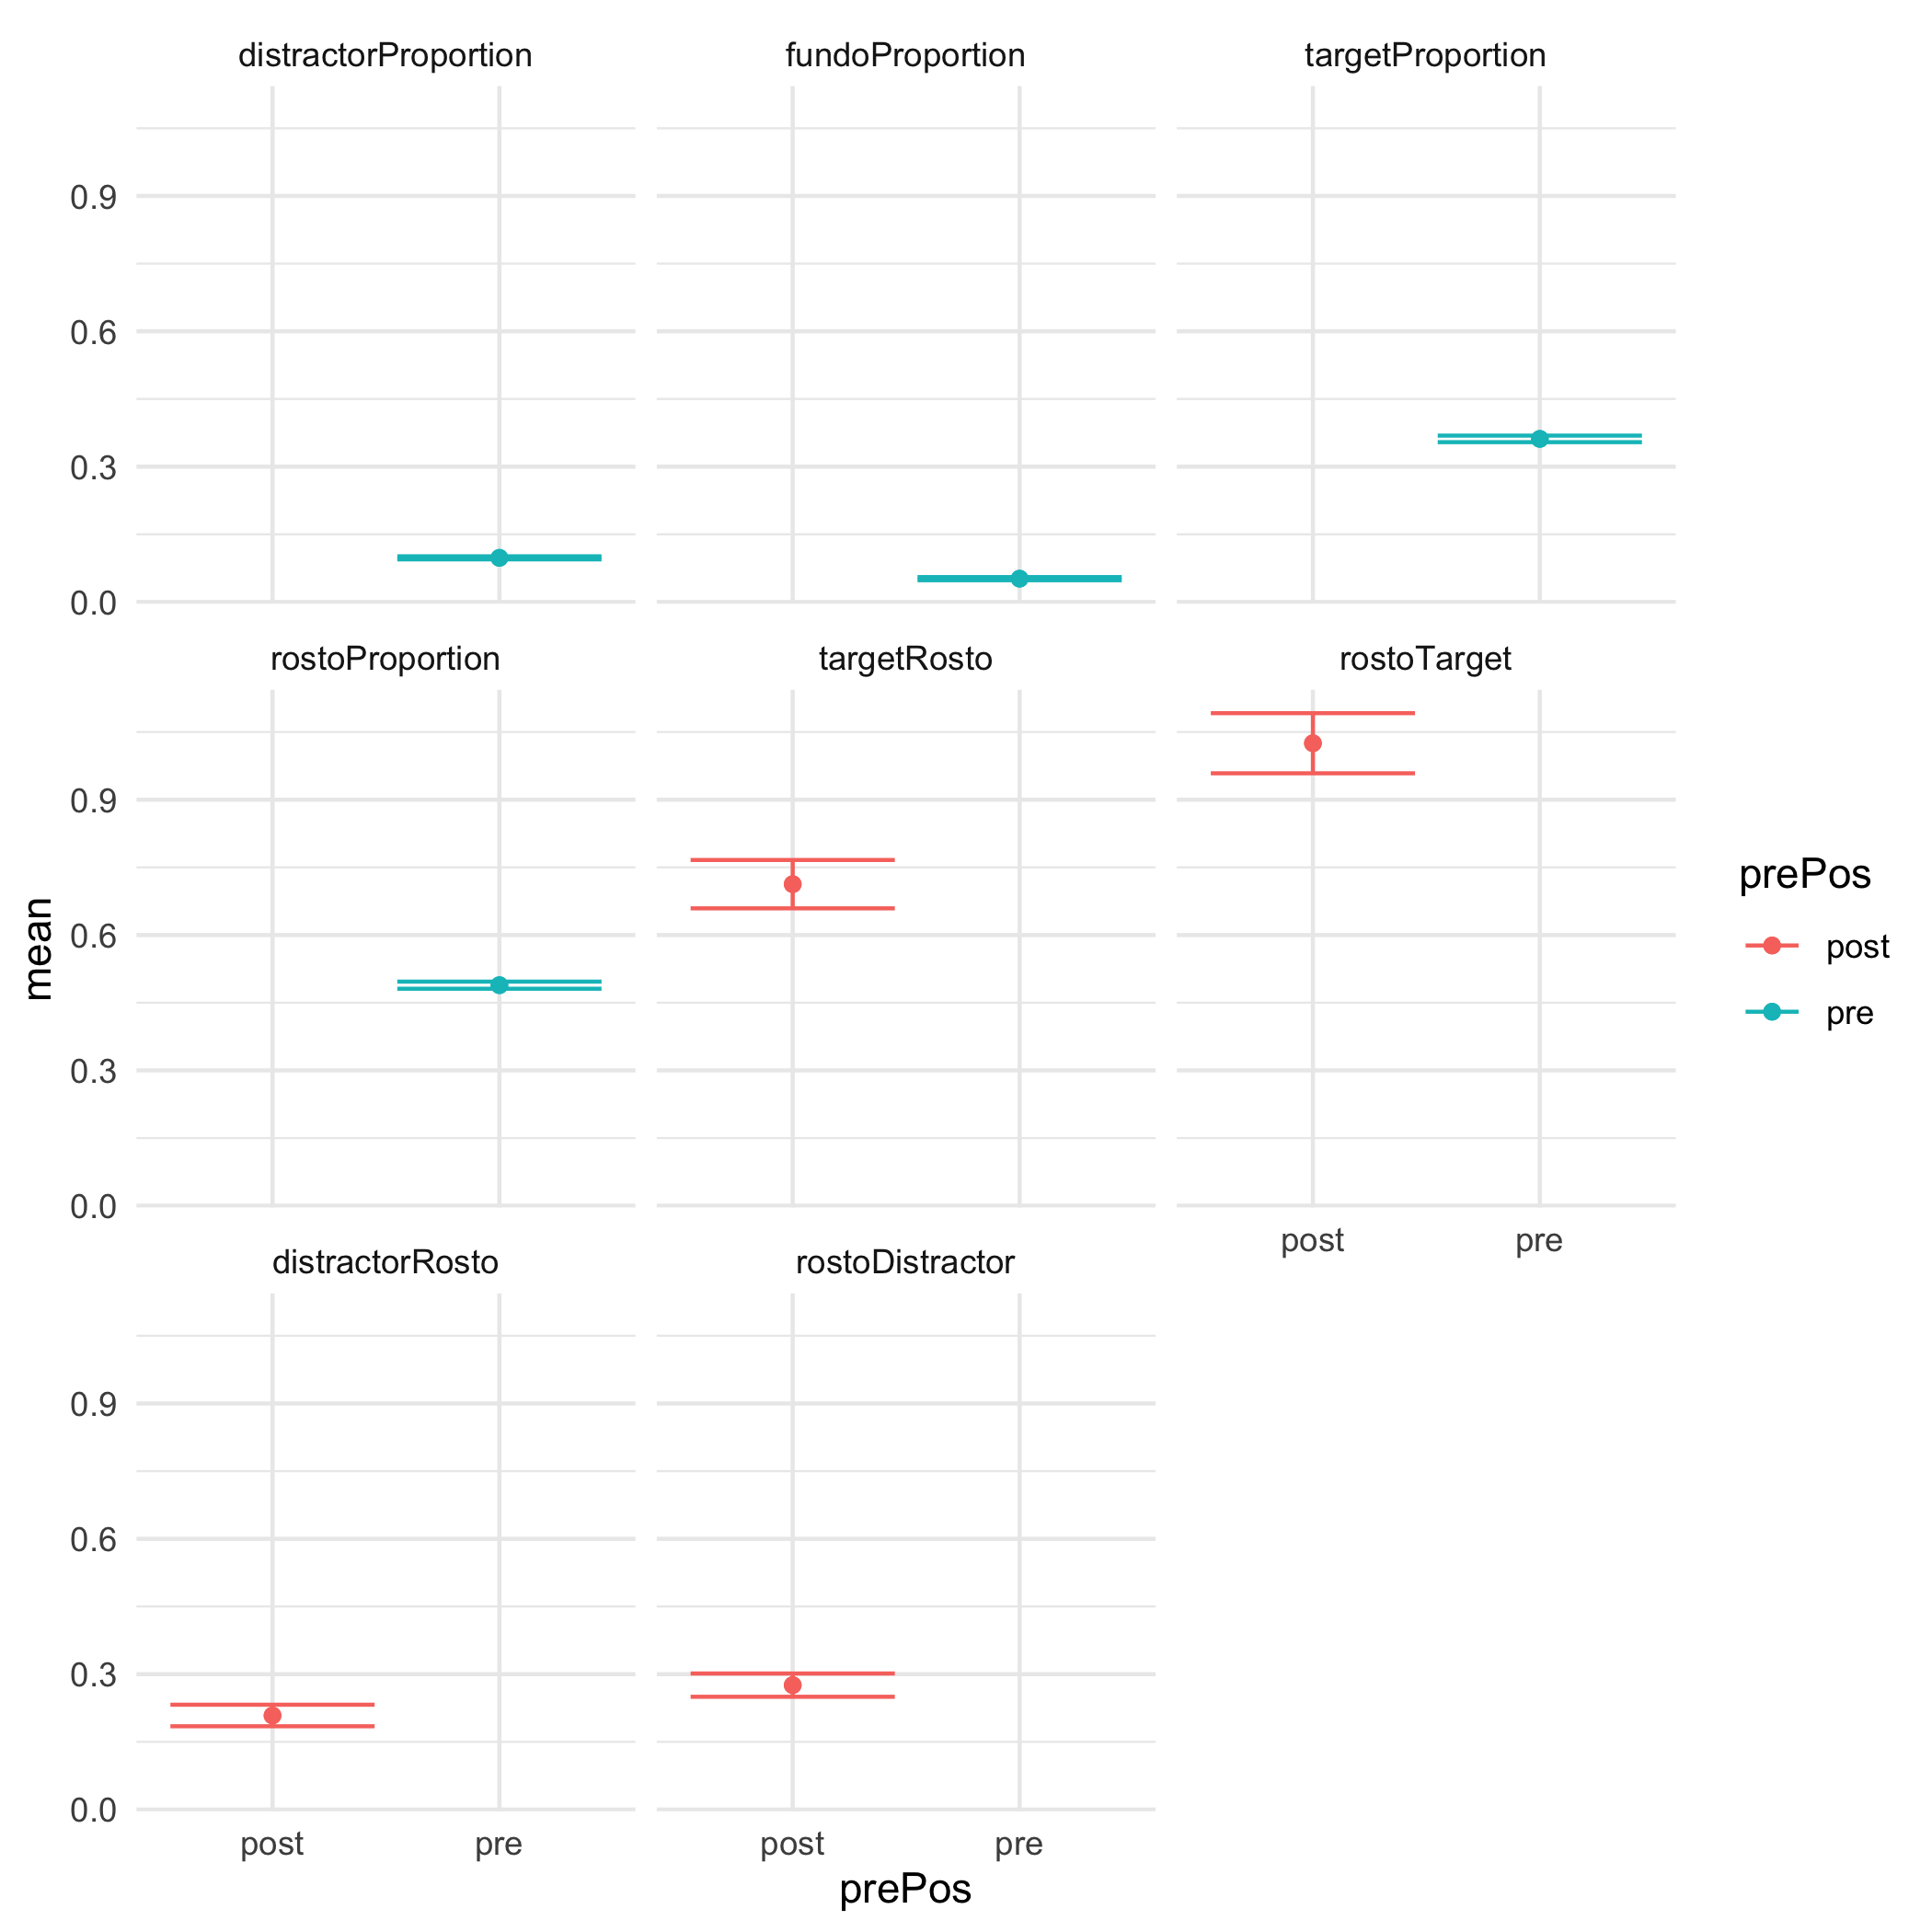
\includegraphics[scale=0.2]{./prePosVarProportion.png}}
  \centering
\end{figure}

\begin{table}[ht]
\centering
\begin{tabular}{rllrr}
  \hline
 & variable & prePos & mean & stder \\ 
  \hline
  1 & distractorProportion & pre & 0.10 & 0.00 \\ 
  2 & fundoProportion & pre & 0.05 & 0.00 \\ 
  3 & targetProportion & pre & 0.36 & 0.01 \\ 
  4 & rostoProportion & pre & 0.49 & 0.01 \\ 
  5 & targetRosto & post & 0.71 & 0.05 \\ 
  6 & rostoTarget & post & 1.03 & 0.07 \\ 
  7 & distractorRosto & post & 0.21 & 0.02 \\ 
  8 & rostoDistractor & post & 0.28 & 0.03 \\ 
   \hline
\end{tabular}
\end{table}

\begin{figure}[H]
  \caption{}
  \noindent\makebox[\textwidth]{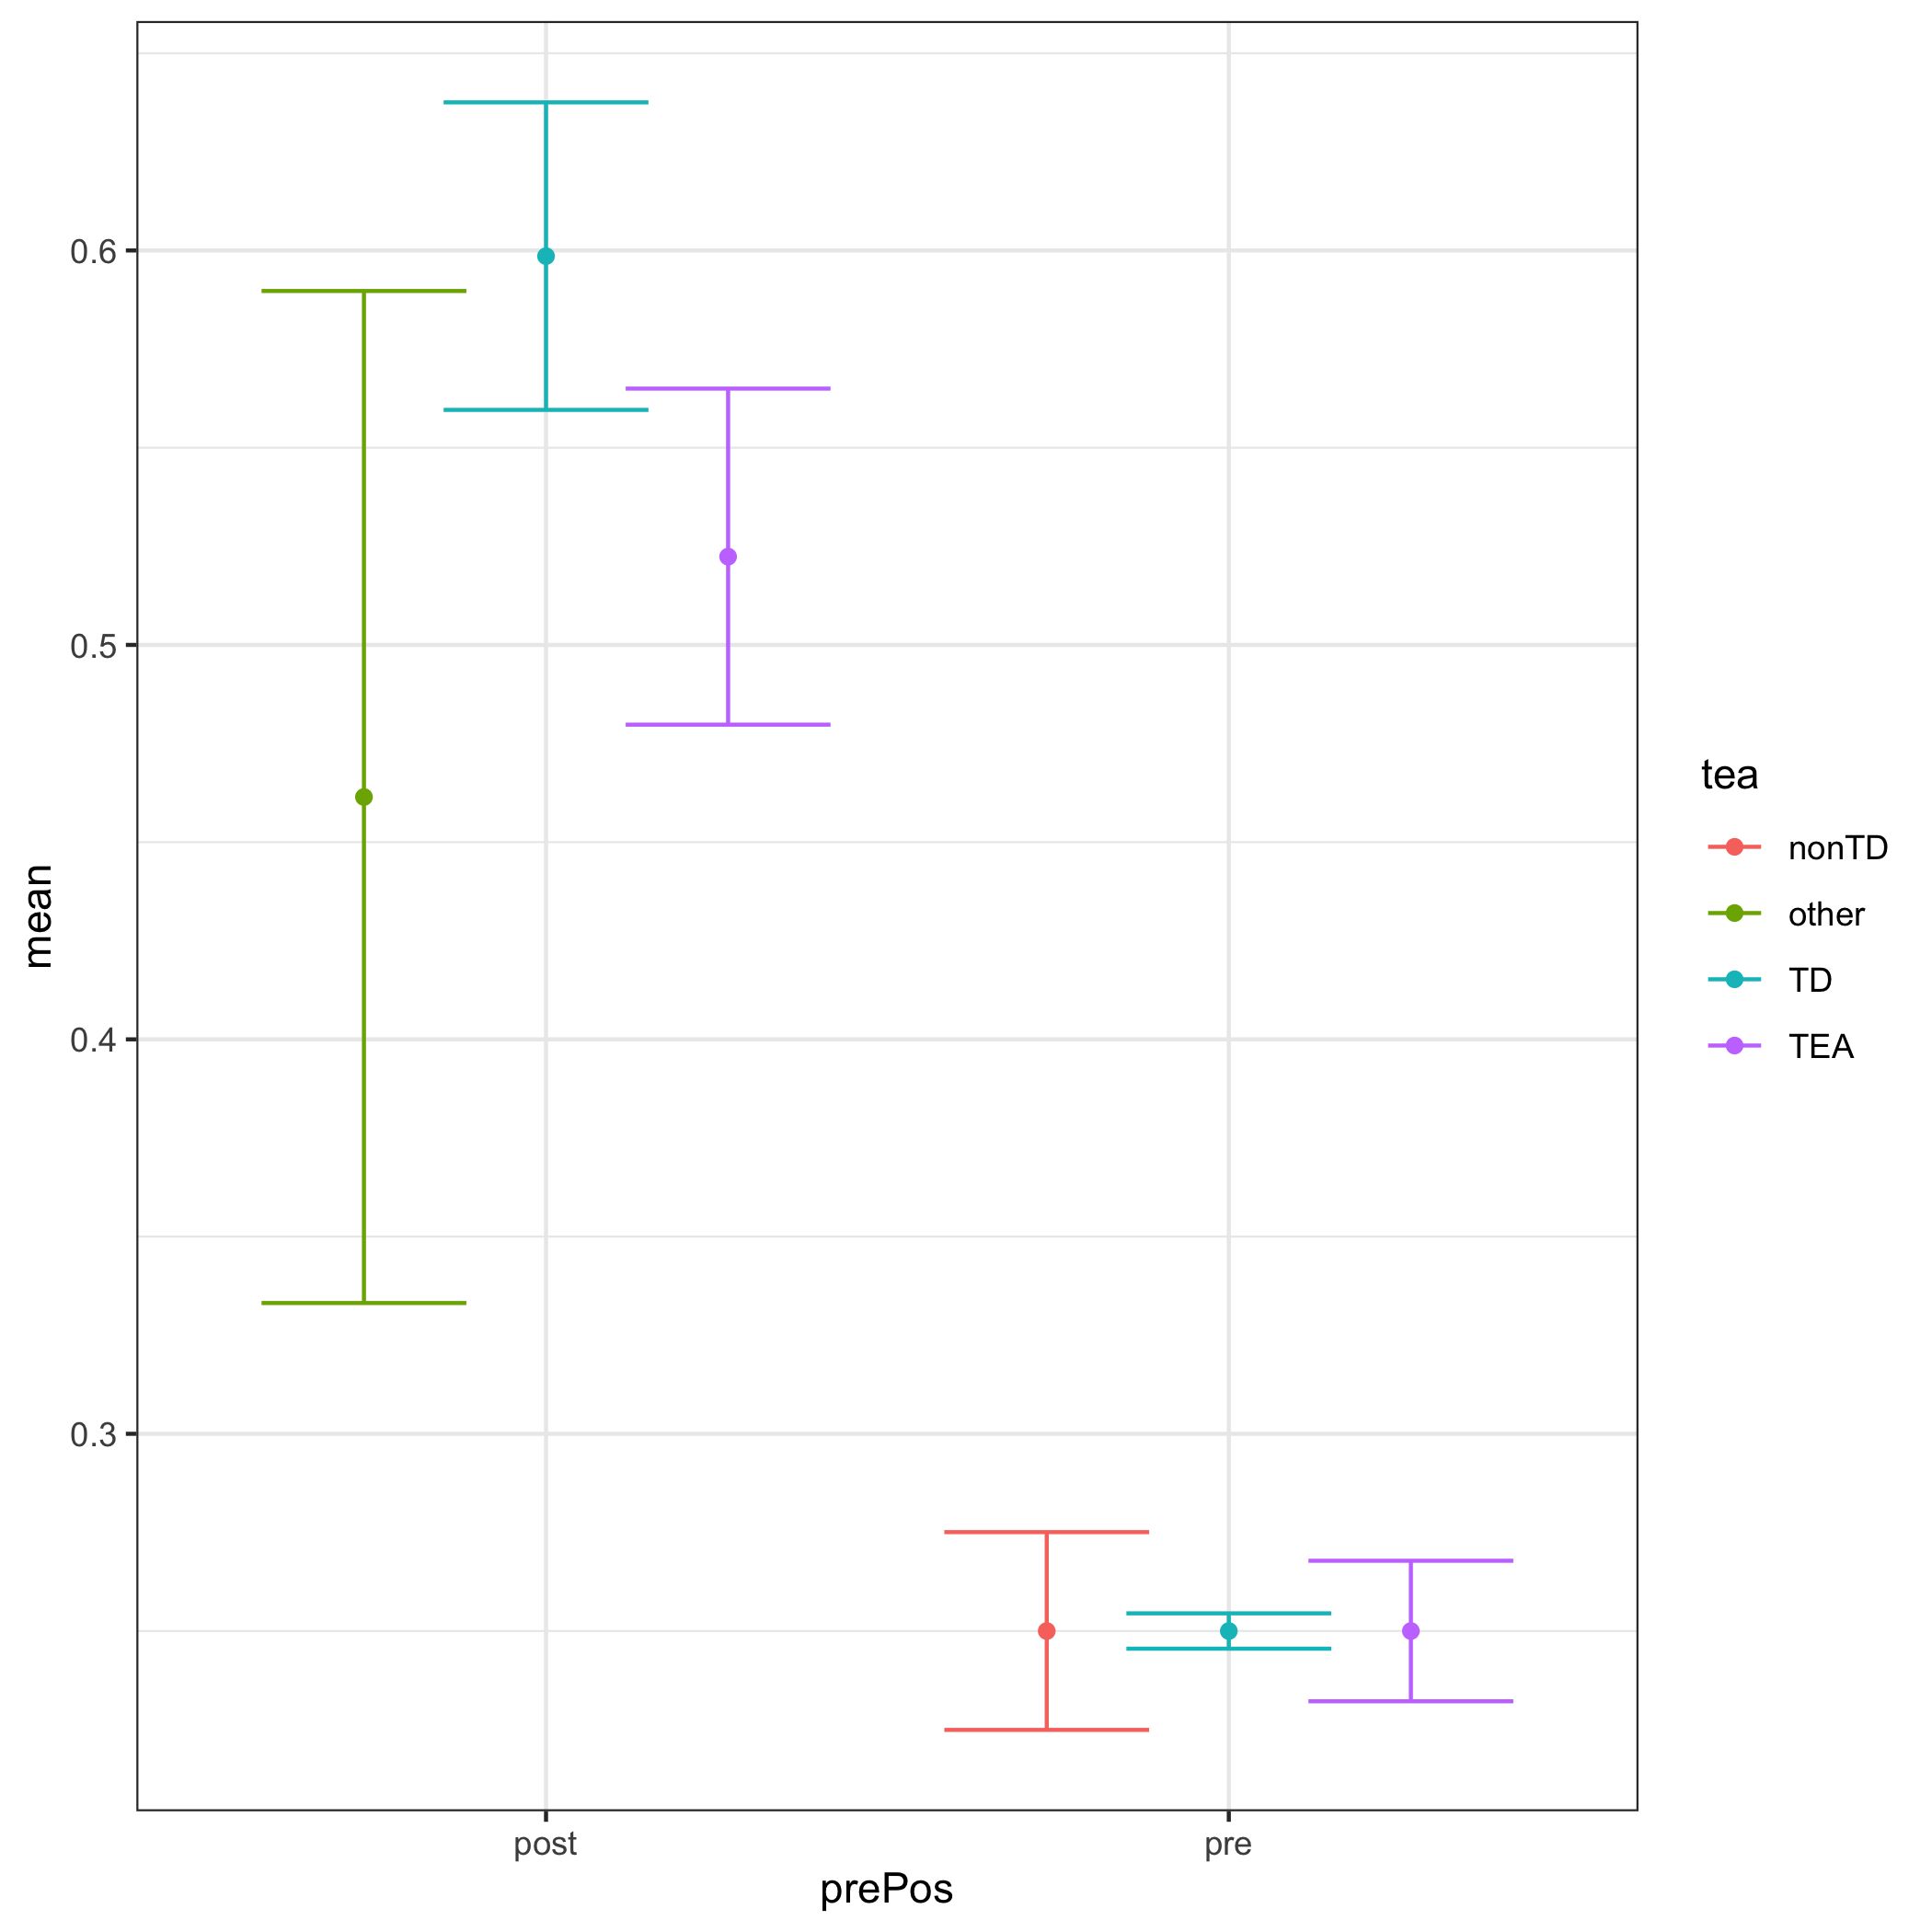
\includegraphics[scale=0.2]{./teaPrePosProportion.png}}
  \centering
\end{figure}

\begin{table}[ht]
\centering
\caption{}
\begin{tabular}{rllrr}
  \hline
 & prePos & tea & mean & stder \\ 
  \hline
1 & post & other & 0.46 & 0.13 \\ 
  2 & post & TD & 0.60 & 0.04 \\ 
  3 & post & TEA & 0.52 & 0.04 \\ 
  4 & pre & nonTD & 0.25 & 0.03 \\ 
  5 & pre & TD & 0.25 & 0.00 \\ 
  6 & pre & TEA & 0.25 & 0.02 \\ 
   \hline
\end{tabular}
\end{table}

\begin{figure}[H]
  \caption{}
  \noindent\makebox[\textwidth]{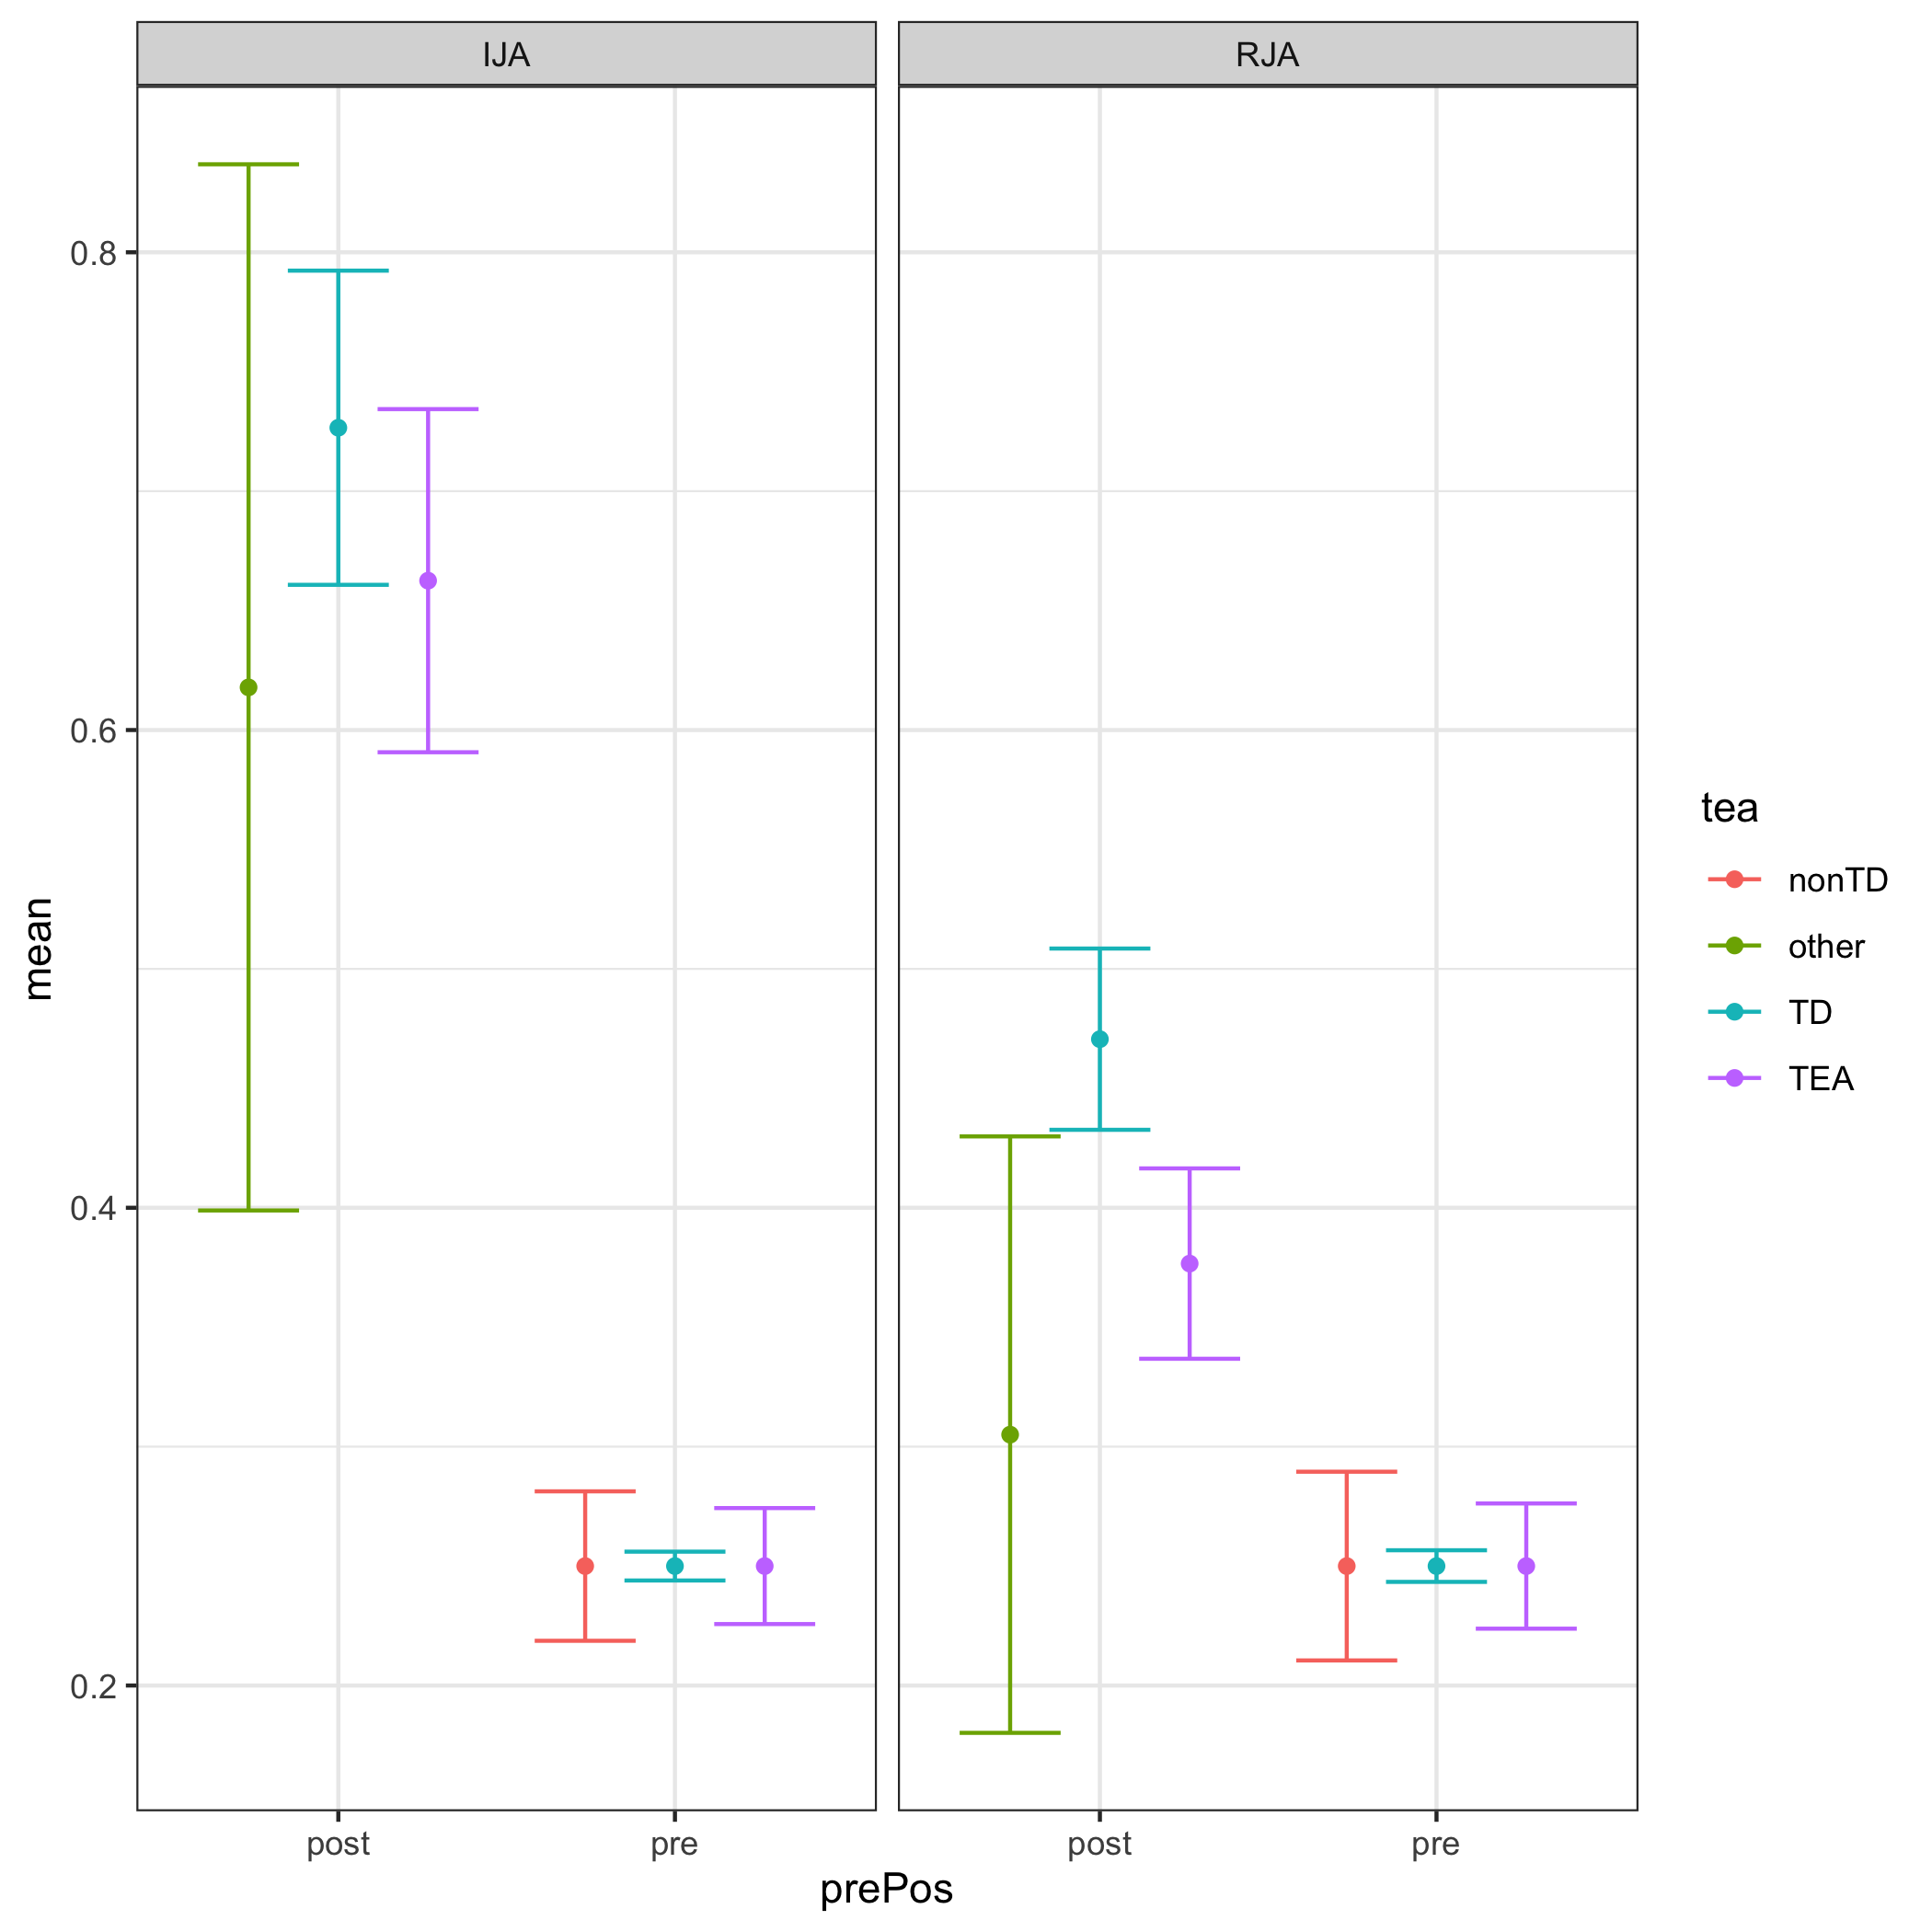
\includegraphics[scale=0.2]{./teaConditionProportion.png}}
  \centering
\end{figure}

\begin{table}[ht]
\centering
\begin{tabular}{rlllrr}
  \hline
 & condition & tea & prePos & mean & stder \\ 
  \hline
1 & IJA & nonTD & pre & 0.25 & 0.03 \\ 
  2 & IJA & other & post & 0.62 & 0.22 \\ 
  3 & IJA & TD & post & 0.73 & 0.07 \\ 
  4 & IJA & TD & pre & 0.25 & 0.01 \\ 
  5 & IJA & TEA & post & 0.66 & 0.07 \\ 
  6 & IJA & TEA & pre & 0.25 & 0.02 \\ 
  7 & RJA & nonTD & pre & 0.25 & 0.04 \\ 
  8 & RJA & other & post & 0.31 & 0.12 \\ 
  9 & RJA & TD & post & 0.47 & 0.04 \\ 
  10 & RJA & TD & pre & 0.25 & 0.01 \\ 
  11 & RJA & TEA & post & 0.38 & 0.04 \\ 
  12 & RJA & TEA & pre & 0.25 & 0.03 \\ 
   \hline
\end{tabular}
\end{table}

\end{document}
